\documentclass[tikz,border=5pt]{standalone}
\usepackage{ctex,amsmath}
\usetikzlibrary{arrows.meta,calc}
\tikzset{>=Latex,wire/.style={blue!70!black,very thick},guide/.style={gray!65,thin},force/.style={orange!85!black,thick,->},field/.style={green!45!black,thick,->}}
\begin{document}
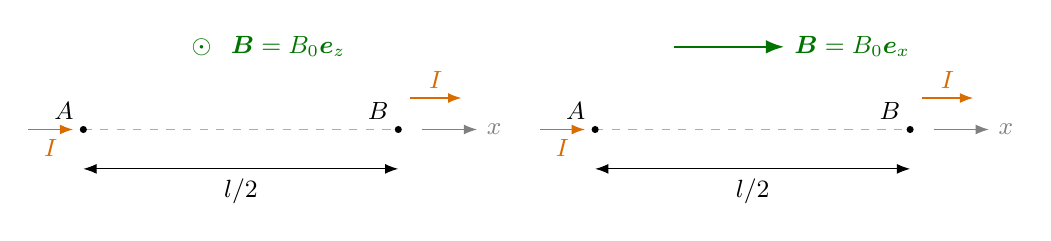
\begin{tikzpicture}[font=\small]
\foreach \q in {0,1}{
\begin{scope}[xshift={6.5*\q cm}]
\draw[guide,dashed](0,0)--(4,0);
\fill(0,0)circle(.045)node[above left]{$A$};
\fill(4,0)circle(.045)node[above left]{$B$};
\draw[->,gray](4.3,0)--(5,0)node[right]{$x$};
\draw[<->](0,-.5)--(4,-.5)node[midway,below]{$l/2$};
\draw[orange!85!black,->](-.7,0)--(-.13,0)node[midway,below]{$I$};
\draw[orange!85!black,->](4.15,.40)--(4.8,.40)node[midway,above]{$I$};
\ifnum\q=0
\node[green!45!black]at(1.5,1.05){$\odot$};
\node[green!45!black,right]at(1.75,1.05){$\boldsymbol B=B_0\boldsymbol e_z$};
\else
\draw[field](1,1.05)--(2.4,1.05)node[right]{$\boldsymbol B=B_0\boldsymbol e_x$};
\fi
\end{scope}}
\end{tikzpicture}
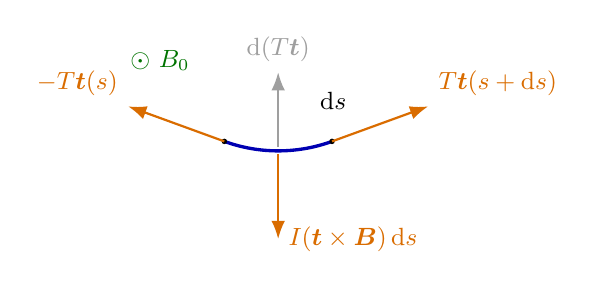
\begin{tikzpicture}[font=\small]
\draw[wire]({2*cos(250)},{2+2*sin(250)})arc[start angle=250,end angle=290,radius=2];
\coordinate(P)at({2*cos(250)},{2+2*sin(250)});
\coordinate(Q)at({2*cos(290)},{2+2*sin(290)});
\fill(P)circle(.035);\fill(Q)circle(.035);
\draw[force](P)--++(160:1.3)node[above left]{$-T\boldsymbol t(s)$};
\draw[force](Q)--++(20:1.3)node[above right]{$T\boldsymbol t(s+\mathrm ds)$};
\draw[force](0,-.04)--(0,-1.12)node[right]{$I(\boldsymbol t\times\boldsymbol B)\,\mathrm ds$};
\draw[gray!75,thick,->](0,.05)--(0,1.00)node[above]{$\mathrm d(T\boldsymbol t)$};
\node[above]at(.7,.40){$\mathrm ds$};
\node[green!45!black]at(-1.5,1.15){$\odot\ B_0$};
\end{tikzpicture}
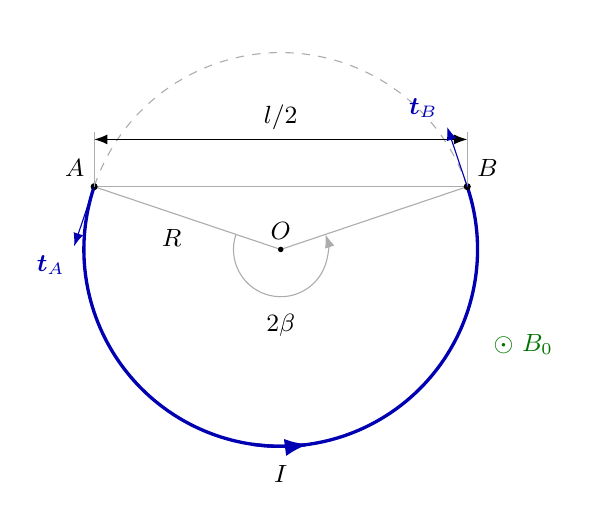
\begin{tikzpicture}[font=\small]
\def\be{108.6038215923}\def\ra{2.5}
\coordinate(A)at(0,0);
\coordinate(B)at({2*\ra*sin(\be)},0);
\coordinate(O)at({\ra*sin(\be)},{\ra*cos(\be)});
\draw[guide,dashed](B)arc[start angle={\be-90},end angle={270-\be},radius=\ra];
\draw[wire]plot[domain=-\be:\be,samples=181] ({\ra*(sin(\x)+sin(\be))},{\ra*(cos(\be)-cos(\x))});
\draw[guide](A)--(B);
\draw[guide](A)--(O)--(B);
\fill(A)circle(.045)node[above left]{$A$};
\fill(B)circle(.045)node[above right]{$B$};
\fill(O)circle(.035)node[above]{$O$};
\node[below left]at($(A)!.52!(O)$){$R$};
\draw[<->](0,.6)--({2*\ra*sin(\be)},.6)node[midway,above]{$l/2$};
\draw[guide](A)--(0,.7)(B)--({2*\ra*sin(\be)},.7);
\draw[blue!70!black,->](A)--++({-\be}:.8)node[below left]{$\boldsymbol t_A$};
\draw[blue!70!black,->](B)--++(\be:.8)node[above left]{$\boldsymbol t_B$};
\draw[guide,->]($(O)+({270-\be}:.6)$)arc[start angle={270-\be},end angle={270+\be},radius=.6];
\node[below]at($(O)+(0,-.70)$){$2\beta$};
\draw[wire,->]plot[domain=-8:8,samples=25] ({\ra*(sin(\x)+sin(\be))},{\ra*(cos(\be)-cos(\x))});
\node[below]at({\ra*sin(\be)},{\ra*(cos(\be)-1)-.12}){$I$};
\node[green!45!black]at(5.45,-2){$\odot\ B_0$};
\end{tikzpicture}
\begin{tikzpicture}[font=\small,x={(.92cm,.04cm)},y={(.55cm,-.32cm)},z={(0cm,.90cm)}]
\def\rr{1.6539866863}
\foreach \a in {0,6}{
\draw[guide,dashed]plot[domain=180:360,samples=80] (\a,{\rr*sin(\x)},{\rr*(1-cos(\x))});
\draw[guide]plot[domain=0:180,samples=80] (\a,{\rr*sin(\x)},{\rr*(1-cos(\x))});
}
\draw[guide](0,0,0)--(6,0,0)(0,0,{2*\rr})--(6,0,{2*\rr});
\draw[gray,dash dot](0,0,\rr)--(6.4,0,\rr);
\node[above]at(6.15,0,\rr){圆柱轴};
\draw[wire]plot[domain=0:180,samples=101] ({\x/60},{\rr*sin(\x)},{\rr*(1-cos(\x))});
\draw[wire,dashed]plot[domain=180:360,samples=101] ({\x/60},{\rr*sin(\x)},{\rr*(1-cos(\x))});
\draw[wire,->]plot[domain=70:85,samples=20] ({\x/60},{\rr*sin(\x)},{\rr*(1-cos(\x))});
\node[left]at(1.2,{\rr*sin(72)},{\rr*(1-cos(72))}){$I$};
\fill(0,0,0)circle(.04)node[below left]{$A$};
\fill(6,0,0)circle(.04)node[below right]{$B$};
\draw[gray,->](6.3,0,0)--(7.2,0,0)node[right]{$x$};
\draw[gray,->](0,0,0)--(0,2.3,0)node[below right]{$y$};
\draw[gray,->](0,0,0)--(0,0,3.9)node[above]{$z$};
\draw[<->](6.75,0,0)--(6.75,0,\rr)node[midway,right]{$r_1$};
\draw[guide,dashed](6.1,0,\rr)--(6.9,0,\rr);
\draw[field](1,0,4.0)--(3,0,4.0)node[right]{$B_0$};
\draw[<->](0,0,-.85)--(6,0,-.85)node[midway,below]{$p_1=l/2$};
\node[below]at(3,0,-.20){$AB$：圆柱母线};
\end{tikzpicture}
\begin{tikzpicture}[font=\small]
\def\pp{2.2}\def\ww{3.81051177665}
\coordinate(A)at(0,0);\coordinate(B)at(\ww,\pp);\coordinate(C)at(\ww,0);
\draw[guide](A)--(\ww,0)--(B)--(0,\pp)--cycle;
\draw[wire,->](A)--(B)node[midway,sloped,above]{$l/n$};
\fill(A)circle(.035)node[below left]{$A$};
\fill(B)circle(.035)node[above right]{$B$};
\draw[<->](0,-.55)--(\ww,-.55)node[midway,below]{$2\pi r_n=\sqrt3 l/(2n)$};
\draw[<->](4.35,0)--(4.35,\pp)node[midway,right]{$p_n=l/(2n)$};
\draw[guide,dashed](\ww,0)--(4.5,0)(B)--(4.5,\pp);
\draw[guide](.65,0)arc[start angle=0,end angle=30,radius=.65];
\node at(1.4,.18){$\alpha'=30^\circ$};
\draw[guide]($(B)+(210:.50)$)arc[start angle=210,end angle=270,radius=.50];
\node at(3.52,1.21){$\alpha=60^\circ$};
\draw[guide](C)++(-.18,0)--++(0,.18)--++(.18,0);
\node[above]at(1.9,2.48){一匝圆柱面展开};
\end{tikzpicture}
\end{document}
